% Copyright 2004 by Till Tantau <tantau@users.sourceforge.net>.
%
% In principle, this file can be redistributed and/or modified under
% the terms of the GNU Public License, version 2.
%
% However, this file is supposed to be a template to be modified
% for your own needs. For this reason, if you use this file as a
% template and not specifically distribute it as part of a another
% package/program, I grant the extra permission to freely copy and
% modify this file as you see fit and even to delete this copyright
% notice. 

\documentclass{beamer}

% There are many different themes available for Beamer. A comprehensive
% list with examples is given here:
% http://deic.uab.es/~iblanes/beamer_gallery/index_by_theme.html
% You can uncomment the themes below if you would like to use a different
% one:
%\usetheme{AnnArbor}
%\usetheme{Antibes}
%\usetheme{Bergen}
%\usetheme{Berkeley}
%\usetheme{Berlin}
%\usetheme{Boadilla}
%\usetheme{boxes}
%\usetheme{CambridgeUS}
%\usetheme{Copenhagen}
%\usetheme{Darmstadt}
%\usetheme{default}
%\usetheme{Frankfurt}
%\usetheme{Goettingen}
%\usetheme{Hannover}
%\usetheme{Ilmenau}
%\usetheme{JuanLesPins}
%\usetheme{Luebeck}
\usetheme{Madrid}
%\usetheme{Malmoe}
%\usetheme{Marburg}
%\usetheme{Montpellier}
%\usetheme{PaloAlto}
%\usetheme{Pittsburgh}
%\usetheme{Rochester}
%\usetheme{Singapore}
%\usetheme{Szeged}
%\usetheme{Warsaw}
%\usepackage{enumitem}

\setbeamertemplate{items}[circle]
\usepackage{tikz}
%%%%%%%%%%%%%%%%%%%%%%%%%%%%%%%%%%%%%%

% frames

%\begin{frame}{Blocks}
%\begin{block}{Block Title}
%You can also highlight sections of your presentation in a block, with it's own title
%\end{block}
%\begin{theorem}
%There are separate environments for theorems, examples, definitions and proofs.
%\end{theorem}
%\begin{example}
%Here is an example of an example block.
%\end{example}
%\end{frame}


%%%%%%%%%%%%%%%%%%%%%%%%%%%%%%%%%%%%%%

%%%%%%%%%%%%%%%%%%%%%%%%%%%%%%%%%%%%%%%%%
% New Command

% Contradiction
\newcommand{\contradiction}{%
  \ensuremath{{(\Rightarrow\mspace{-2mu}\Leftarrow)}}%
}

% Norm
\newcommand{\norm}[1]{\left\lVert#1\right\rVert}

% Distance
\newcommand{\dist}{\text{dist}}

% Proximal map
\newcommand{\prox}{\text{prox}}

% argmax argmin
\DeclareMathOperator*{\argmax}{argmax}
\DeclareMathOperator*{\argmin}{argmin}

% enumerate numbering
\newcommand\mynum[1]{%
  \usebeamercolor{enumerate item}%
  \tikzset{beameritem/.style={circle,inner sep=0,minimum size=2ex,text=enumerate item.bg,fill=enumerate item.fg,font=\footnotesize}}%
  \tikz[baseline=(n.base)]\node(n)[beameritem]{#1};%
}

%%%%%%%%%%%%%%%%%%%%%%%%%%%%%%%%%%%%%%%%%

\title{Application of Particle Swarm Optimization\\ in minimax D-optimal Design}

% A subtitle is optional and this may be deleted
%\subtitle{MM Optimization Algorithms}

\author{Park, Sungmin}
% - Give the names in the same order as the appear in the paper.
% - Use the \inst{?} command only if the authors have different
%   affiliation.

\institute[SNU] % (optional, but mostly needed)
{
  Department of Statistics\\
  Seoul National University
}
% - Use the \inst command only if there are several affiliations.
% - Keep it simple, no one is interested in your street address.

\date{10 MAY 19}
% - Either use conference name or its abbreviation.
% - Not really informative to the audience, more for people (including
%   yourself) who are reading the slides online

\subject{Computational Statistics}
% This is only inserted into the PDF information catalog. Can be left
% out. 

% If you have a file called "university-logo-filename.xxx", where xxx
% is a graphic format that can be processed by latex or pdflatex,
% resp., then you can add a logo as follows:

% \pgfdeclareimage[height=0.5cm]{university-logo}{university-logo-filename}
% \logo{\pgfuseimage{university-logo}}

% Delete this, if you do not want the table of contents to pop up at
% the beginning of each subsection:
%\AtBeginSubsection[]
\AtBeginSection[]
{
  \begin{frame}<beamer>{Outline}
    \tableofcontents[currentsection,currentsubsection]
  \end{frame}
}

% Let's get started
\begin{document}

\begin{frame}
  \titlepage
\end{frame}

\begin{frame}{Outline}
  \tableofcontents
  % You might wish to add the option [pausesections]
\end{frame}

% Section and subsections will appear in the presentation overview
% and table of contents.

\section{Introduction}
\begin{frame}
  Optimal design for nonlinear model is an optimization problem where analytical formula for the design is rarely available.\\
  \vspace{3mm}
  In this session,
  \vspace{3mm}
  \begin{itemize}
    \item Locally D-optimal design is generalized to minimax D-optimal design.
    \vspace{3mm}
    \item Particle swarm optimization is applied to minimax D-optimal design.
    \vspace{3mm}
    \item Limitations of particle swarm optimization are discussed.
  \end{itemize}
\end{frame}

\section{Minimax D-optimal Design}

%\subsection{Regression}

%% 1
\begin{frame}{Review}%{Optional Subtitle}
  Given
  \begin{itemize}
    \item $\mathcal{P}(\cdot)$: model
    \item $\theta$: parameter
    \item $k$: \# of distinct design points
  \end{itemize}
  \vspace{3mm}
  find 
  \begin{itemize}
    \item $x_i$: design points
    \item $w_i$: proportion of subjects assigned to design point $x_i$
    \item[] i.e. $\xi = \left\{ (x_i,w_i) : i=1,\ldots,k \right\}$: k-point approximate design
  \end{itemize}
  \vspace{3mm}
  s.t. minimizes
  \begin{flalign*}
       \left| Var \left( \hat{\theta}(\xi) \right) \right| \hspace{3mm} (D \text{-optimality criterion})
    \end{flalign*}
\end{frame}

\begin{frame}{Review}%{Optional Subtitle}
  More specifically using MLE,
  \begin{itemize}
    \item $\mathcal{P}(\cdot)$: model
    \item $\theta$: parameter
    \item $k$: \# of distinct design points
  \end{itemize}
  \vspace{3mm}
  find 
  \begin{itemize}
    \item $x_i$: design points
    \item $w_i$: proportion of subjects assigned to design point $x_i$
    \item[] i.e. $\xi = \left\{ (x_i,w_i) : i=1,\ldots,k \right\}$: k-point approximate design
  \end{itemize}
  \vspace{3mm}
  s.t. minimizes
  \begin{flalign*}
       -log \hspace{1mm} det \left( \mathcal{I} \left( \xi,\theta \right) \right)  , \hspace{3mm} \mathcal{I} \left( \xi, \theta \right) \text{: Fisher information}
    \end{flalign*}
\end{frame}

%% 4
\begin{frame}{Minimax D-optimal design}
    In locally D-optimal design, nominal value of $\theta_0$ is given.
    \vspace{3mm}
    \begin{flalign*}
      & \xi^{*} =  \argmin_{\xi} \left\{\hspace{1mm} -log \hspace{1mm} det \left( \mathcal{I} \left( \xi, \theta_0 \right) \right) \hspace{1mm}\right\} \hspace{1mm} \text{for some fixed } \theta_0
    \end{flalign*}\\
    \vspace{6mm}
    In minimax D-optimal design, parameter space $\Theta$ is given.\\
    \vspace{2mm}
    \hspace{0mm} Corresponding optimality criterion is defined as,
    \vspace{3mm}
    \begin{flalign*}
      & \xi^{*} =  \argmin_{\xi} \max_{\theta \in \Theta} \left\{\hspace{1mm} -log \hspace{1mm} det \left( \mathcal{I} \left( \xi,\theta \right) \right) \hspace{1mm}\right\}
    \end{flalign*}
\end{frame}

%% 7
\begin{frame}{Equivalence Theorem}
  \begin{theorem}[Berger et al., 2000][Notation]
    \begin{itemize}
      \item $\mathcal{X}$ : design space, $\xi = \left\{ (x_i,w_i) : i=1,\ldots,k \right\}, x_i \in \mathcal{X}$
      \item $\Theta$ : parameter space, $\theta \in \Theta$
      \item $\mathcal{I}(x,\theta)$ : Fisher information at observation point $x$
      \item $\mathcal{I}(\xi,\theta) = \int \mathcal{I}(x,\theta) \xi(dx)$ : Fisher information of design $\xi$
      \item[] $\ast$ Recall: design $\xi$ is a probability measure.
    \end{itemize}
  \end{theorem}
\end{frame}
  
%% 7
\begin{frame}{Equivalence Theorem}
  \begin{theorem}[Berger et al., 2000]
  Suppose the design space $\mathcal{X}$ and parameter space $\Theta$ are known compact spaces and $q$ is the number of parameters in the model. The following statements are equivalent:
    \begin{flalign*}
      1.\hspace{2mm} &\xi^{*} =  \argmin_{\xi} \max_{\theta \in \Theta} \left\{ -log \hspace{1mm} det \left( \mathcal{I} \left( \xi,\theta \right) \right) \right\}\\
      2.\hspace{2mm} &\forall \xi \in \mathcal{X}, \min_{\theta \in A(\xi^*)}\int_{\Theta}tr \hspace{1mm} \mathcal{I}^{-1}(\xi^*,\theta)\mathcal{I}(x,\theta)\xi(dx) - q \leq 0, \text{ where}\\
      &A(\xi) = \left\{ \theta^* \in \Theta : -log \hspace{1mm} det \left( \mathcal{I} \left( \xi,\theta^* \right) \right) = \max_{\theta \in \Theta}  \left\{ -log \hspace{1mm} det \left( \mathcal{I} \left( \xi,\theta \right) \right) \right\} \right\}\\
      3.\hspace{2mm} &\exists \text{ probability measure } \gamma^* \text{ on } A(\xi^*) \hspace{2mm} s.t.\\
      &\int_{A(\xi^*)}tr \hspace{1mm} \mathcal{I}^{-1}(\xi^*,\theta)\mathcal{I}(x,\theta)\gamma^*(d\theta) - q \leq 0, \forall \theta \in \Theta \\
    \end{flalign*}
  \end{theorem}
\end{frame}

\begin{frame}{Equivalence Theorem}
  Although equivalence theorem provides an alternative to check the optimality of the design, $A(\xi)$ and $\gamma^*$ defined on $A(\xi^*)$ are unknown.\\
  \vspace{6mm}
  Verifying the inequality in equivalence theorem requires solving yet another optimization problem.
\end{frame}

\section{PSO in Minimax Optimization}

%% 9 
\begin{frame}{Particle Swarm Optimization}
  Particle Swarm Optimization (PSO) is a nature-inspired algorithm originating from research in fish and swarm movement behavior.\\
  \vspace{3mm}
  Benefits of PSO include the ability to find the optimal solution to a complex problem or get close to the optimal solution quickly \textbf{without requiring any assumption on the objective function}. $\Rightarrow$ \textbf{flexible}\\
  \vspace{3mm}
  However, the method still lacks a firm theoretical justification to date\\
  and is under-utilized in statistical literature. (Qui et al., 2014)\\
  \vspace{3mm}
  The idea of PSO is as follows,\\
  \begin{enumerate}
    \item A number of particles are scattered onto the search domain.
    \item Each particle investigates the search domain and shares knowledge with the group.
    \item Possible solution is obtained from the group's aggregated knowledge.
  \end{enumerate}
\end{frame}

%%10
\begin{frame}{PSO Algorithm}
  Update Equation:\\
  \begin{flalign}
    v_i^{t+1} &= \tau_t v_i^t + \gamma_1 \beta_1 \odot (p_i^t-z_i^t)+ \gamma_2 \beta_2 \odot (p_g^t-z_i^t),\\
    z_i^{t+1} &= z_i^t + v_i^{t+1}.
  \end{flalign}
  \begin{itemize}
    \item $h(\cdot)$: objective function (fitness) to minimize
    \item $z_i^t$: position of the $i$th particle at time $t$
    \item $v_i^t$: velocity of the $i$th particle at time $t$
    \item $p_i^t$: $\argmin_{z_i^s, 1 \leq s \leq t} \left\{ h(z_i^s) \right\}$, personal best position
    \item $p_g^t$: $\argmin_{z_m^s, 1 \leq m \leq n, 1 \leq s \leq t} \left\{ h(z_m^s) \right\}$, global best position
    \item $\odot$: Hadamard product operator
  \end{itemize}
\end{frame}

%%11
\begin{frame}{PSO Algorithm}
  Update Equation:\\
  \begin{flalign*}
    v_i^{t+1} &= \tau_t v_i^t + \gamma_1 \beta_1 \odot (p_i^t-z_i^t)+ \gamma_2 \beta_2 \odot (p_g^t-z_i^t),\\
    z_i^{t+1} &= z_i^t + v_i^{t+1}.
  \end{flalign*}
  \begin{itemize}
    \item $\tau_t$: inertia wieght at time $t$, const. or decreasing between (0,1)
    \item $\gamma_1$: cognitive learning parameter
    \item $\gamma_2$: social learning parameter
    \item $\beta_1, \beta_2$: random vector
  \end{itemize}
  \vspace{3mm}
  In this paper, learning parameter was $\gamma_1=\gamma_2=2$ fixed and components of $\beta_1, \beta_2$ was sampled i.i.d from $U(0,1)$ at each iteration and particle.
\end{frame}

%%12
\begin{frame}{PSO Algorithm (1) - Simple PSO}
  PSO pseudo-code for flock size $n$ (i.e. $n$ particles in the swarm)
  \begin{flalign*}  
    \text{(1) }&\text{Initialize particles}\\
    &\text{(1.1) Initiate position } x_i^0 \text{ and velocities } v_i^0 \text{ for } i=1,\ldots,n\\
    &\text{(1.2) Calculate the fitness values } h(x_i^0) \text{ for } i=1,\ldots,n\\
    &\text{(1.3) Determine the personal best positions } p_i^0=x_i^0\\
    &\text{and the global position } p_g^0 \text{ for } i=1,\ldots,n\\
    \text{(2) }&\text{Repeat until stopping criteria are satisfied,}\\
    &\text{(2.1) Calculate particle velocity according to Eq. (1)}\\
    &\text{(2.2) Update particle position according to Eq. (2)}\\
    &\text{(2.3) Project particle back to the design space}\\
    &\text{(2.4) Calculate the fitness values } h(x_i) \text{ for } v_i \text{ for } i=1,\ldots,n\\
    &\text{(2.5) Update personal and global best positions } p_i, (1 \leq i \leq n) \text{ and } p_g\\
    \text{(3) }&\text{Output } p_g = \argmin_x\left\{ h(x) \right\} \text{with \emph{gbest}}=h(p_g)
  \end{flalign*}
\end{frame}

\begin{frame}{Minimax Optimization Problem}
  Let $g(u,v)$ be a given function defined on two compact spaces $\mathcal{U}$ and $\mathcal{V}$.\\
  \vspace{3mm}
  Minimax optimization probelms have the form:
  \begin{flalign*}
    &\min_{u \in \mathcal{U}} \max_{v \in \mathcal{V}} g(u,v) = \min_{u \in \mathcal{U}} f_{outer}(u) =  \min_{u \in \mathcal{U}} \left[ \max_{v \in \mathcal{V}} f_{inner}(v;u) \right] \\
    &\text{ where } f_{outer}(u) =  \max_{v \in \mathcal{V}} f_{inner}(v;u)\\
    &\text{ and, for fixed } u, f_{inner}(v;u) = g(u,v)\\
  \end{flalign*}
\end{frame}

\begin{frame}{Minimax Optimization Problem}
  Let $g(u,v)$ be a given function defined on two compact spaces $\mathcal{U}$ and $\mathcal{V}$.\\
  \vspace{3mm}
  Minimax optimization probelms have the form:
  \begin{flalign}
    &\min_{u \in \mathcal{U}} \max_{v \in \mathcal{V}} g(u,v) = \min_{u \in \mathcal{U}} f_{outer}(u) =  \min_{u \in \mathcal{U}} \left[ \max_{v \in \mathcal{V}} f_{inner}(v;u) \right] 
  \end{flalign}
  where
  \begin{flalign}
    &f_{outer}(u) =  \max_{v \in \mathcal{V}} f_{inner}(v;u)
  \end{flalign}
  and, for fixed $u$,
  \begin{flalign}
    &f_{inner}(v;u) = g(u,v)
  \end{flalign}
\end{frame}

\begin{frame}{PSO Algorithm (2) - Nested PSO}
  Nested PSO pseudo-code for flock size $n$
  \begin{flalign*}  
    \text{(1) }&\text{Initialize particles}\\
    &\text{(1.1) Initiate position } x_i^0 \text{ and velocities } v_i^0 \text{ for } i=1,\ldots,n\\
    &\text{(1.2) Calculate } f_{outer}(x_i) \text{ via Algorithm (1) \color{red} (Inner loop) } \\
    &\text{(1.3) Determine personal and global best positions } p_i, p_g \\
    \text{(2) }&\text{Repeat until stopping criteria are satisfied, \color{red} (Outer loop)}\\
    &\text{(2.1) Calculate particle velocity with Eq. (1)}\\
    &\text{(2.2) Update particle position with Eq. (2)}\\
    &\text{(2.3) Project particle back to design space}\\
    &\text{(2.4) Calculate } f_{outer}(x_i) \text{ via Algorithm (1) \color{red} (Inner loop) } \\
    &\text{(2.5) Update personal and global best positions } p_i, p_g \\
    \text{(3) }&\text{Output } p_g = \argmin_{u \in \mathcal{U}}\left\{ f_{outer}(u) \right\} \text{with \emph{gbest}}=f_{outer}  (p_g)
  \end{flalign*}
\end{frame}

\section{Examples and Discussions}

%%15
\begin{frame}{Compartment Model, locally D-optimal design}
  Example 1: Compartment Model, locally D-optimal design (revisited)\\
  \vspace{3mm}
  Drug concentration$\left(Y\right)$ is modeled as a function$\left(\eta(\cdot,\theta)\right)$ of time$\left(x\right)$\\
  with independent normal errors$\left(\varepsilon \sim \mathcal{N}(0,\sigma^2)\right).$
  \begin{flalign*}
    &Y \sim \mathcal{N}\left(\eta(x,\theta),\sigma^2\right), \sigma^2 : known \\
    \vspace{3mm}
    &\eta(x,\theta)=\theta_3 \left\{ \exp(-\theta_2x)-\exp(-\theta_1x) \right\}, x>0\\
  \end{flalign*}
\end{frame}

%%16
\begin{frame}{Compartment Model, locally D-optimal design}
  \begin{itemize}
    \item $\theta_0 = (0.05884, 4.298, 21.8)$
    \item $n\text{ (flock size)}=100$
    \item $\text{max iteration} = 100$
    \item $k=3$
    \item $\xi = \left\{ (x_i,w_i) : i=1,\ldots,k \right\},$\\
    $x_i \in [0,30], w_i \geq 0, \forall i \text{ and } \sum_{i=1}^k w_i = 1$
  \end{itemize}
  \vspace{3mm}
  $\Rightarrow$ $\xi^*=(0.228773, 1.38858, 18.4168, 0.333335, 0.333332, 0.333333)$
\end{frame}

%%17
\begin{frame}{Compartment Model, locally D-optimal design}
  Equivalence plot for $D$-optimal design:\\
  \vspace{3mm}
  $\left(\frac{\partial \eta(x;\theta)}{\partial\theta}\Big|_{\theta=\theta_0}\right)^T I(\xi^*;\theta_0)^{-1} \left(\frac{\partial \eta(x;\theta)}{\partial\theta}\Big|_{\theta=\theta_0}\right) - 3 \leq 0 , \forall x \in [0,30]$
  \begin{center}
    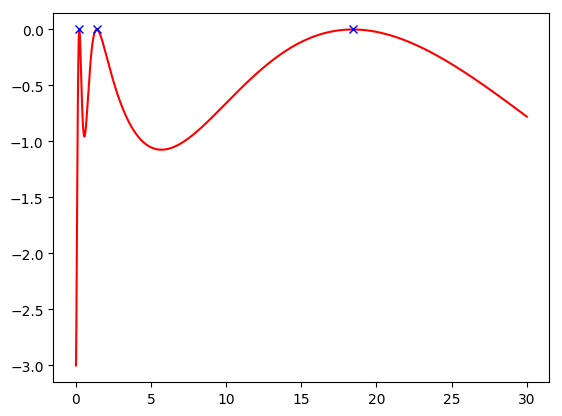
\includegraphics[scale=0.5]{equivplot.png}
  \end{center}
\end{frame}

\begin{frame}{Stability}
  $-log \hspace{1mm} det \left( \mathcal{I} \left( \xi,\theta_0 \right) \right)$ from 1000 simulation arranged in ascending order\\
  \begin{columns}
    \column{0.55\textwidth}
    \begin{center}
      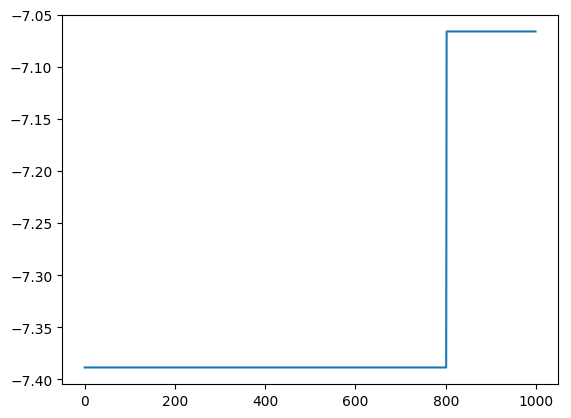
\includegraphics[scale=0.5]{stability.png}
    \end{center}
    \column{0.45\textwidth}
    \begin{itemize}
      \item[*] Relative Efficiency : $RE(\xi) =  \frac{\lvert Cov(\hat{\beta}(\xi^*))\rvert}{\lvert Cov(\hat{\beta}(\xi))\rvert} $ 
      \item 20\% of simulation failed
      \item RE (failed case) = 0.71
    \end{itemize}
  \end{columns}
\end{frame}

\begin{frame}{Two-parameter Logistic Regression Model}
  Example 2: Two-parameter Logistic Regression Model\\
  \hspace{18mm} Minimax D-optimal design\\
  \vspace{3mm}
  \begin{flalign*}
    &Y \sim Ber\left( p(x,\theta) \right) \\
    \vspace{3mm}
    &logit(p(x,\theta)) = -b(x-a),\hspace{3mm} \theta= (a,b)^T\\
  \end{flalign*}
  \begin{flalign*}
    &\text{Find} \hspace{5mm} \xi^{*} =  \argmin_{\xi \in \mathcal{X}} \max_{\theta \in \Theta} \left\{\hspace{1mm} -log \hspace{1mm} det \left( \mathcal{I} \left( \xi,\theta \right) \right) \hspace{1mm}\right\}
  \end{flalign*}
\end{frame}

\begin{frame}{Two-parameter Logistic Regression Model}
  \begin{flalign*}
    \mathcal{I} \left( \xi,\theta \right) &= \int \begin{pmatrix} b^2 & -b(x-a)\\ -b(x-a) & (x-a)^2\\ \end{pmatrix} p(x,\theta)(1-p(x,\theta))d\xi(x) \\
    \left| \mathcal{I} \left( \xi,\theta \right) \right| &=  \sum_{i=1}^{k}w_i p(x_i,\theta)(1-p(x_i,\theta))\\
    &\hspace{5mm} \times \sum_{i=1}^{k} w_i \left\{b(x_i-a)\right\}^2 p(x_i,\theta)(1-p(x_i,\theta))\\
    &\hspace{5mm} - \left\{ \sum_{i=1}^{k} w_i b(x_i-a)^2 p(x_i,\theta)(1-p(x_i,\theta)) \right\} \\
    \ast p(x_i,\theta) &= 1 - p(2a-x_i,\theta)
  \end{flalign*}
\end{frame}

\begin{frame}{Two-parameter Logistic Regression Model}
  Above equations have useful implications when $\Theta = \left[a_L,a_U\right]\times\left[b_L,b_U\right]$.\\
  \vspace{6mm}
  Let $a_M = \frac{1}{2}(a_L+a_U)$.\\
  \vspace{3mm}
  Given a design $\xi = \left\{ (x_i,w_i) : i=1,\ldots,k \right\}$, consider a mirrored design $\xi^s = \left\{ (2a_M-x_i,w_i) : i=1,\ldots,k \right\}$.\\
  \vspace{3mm}
  $\left| \mathcal{I} \left( \xi,\theta \right) \right| = \left| \mathcal{I} \left( \xi^s,\theta \right) \right|$, $\frac{1}{2}(\xi+\xi^s)$ is also optimal for minimax D-optimal $\xi$.\\
  \vspace{6mm}
  $\therefore$ \hspace{1mm} Minimax D-optimal design $\xi^*$ is symmetric about $a_M$.\\
\end{frame}

\begin{frame}{Two-parameter Logistic Regression Model}
  Consider two cases,\\
  \vspace{3mm}
  \begin{itemize}
    \item[(a)] $\Theta=\left[0,2.5\right]\times\left[1,3\right],\mathcal{X}=\left[-1,4\right], k=4$
    \item[(b)] $\Theta=\left[0,3.5\right]\times\left[1,3.5\right],\mathcal{X}=\left[-5,5\right], k=6$
  \end{itemize}
  \vspace{3mm}
  Minimax D-optimal design are presented in King and Wong (2000).
  \vspace{3mm}
  \begin{itemize}
    \item[(a)] support: -0.429, 0.629, 1.871, 2.929
    \item[] weight: 0.245, 0.255, 0.255, 0.245
    \item[(b)] support: -0.35, 0.62, 1.39, 2.11, 2.88, 3.85
    \item[] weight: 0.18, 0.21, 0.11, 0.11, 0.21, 0.18
  \end{itemize}
  \vspace{3mm}
  Note the designs are symmetric.
\end{frame}

\begin{frame}{Nested PSO for minimax D-optimal design}
  We use nested PSO to find minimax D-optimal design for these two cases.\\
  \vspace{3mm}
  For case (a),\\
  \vspace{3mm}
  \begin{itemize}
    \item \makebox[2cm][l]{Outer loop} \# of particles: 32
    \item[] \makebox[2cm][l]{} \# of iterations: 100
    \vspace{3mm}
    \item \makebox[2cm][l]{Inner loop} \# of particles: 64
    \item[] \makebox[2cm][l]{} \# of iterations: 50
  \end{itemize}
\end{frame}

\begin{frame}{Nested PSO for minimax D-optimal design}
  For case (b),\\
  \vspace{3mm}
  \begin{itemize}
    \item \makebox[2cm][l]{Outer loop} \# of particles: 512
    \item[] \makebox[2cm][l]{} \# of iterations: 200
    \vspace{3mm}
    \item \makebox[2cm][l]{Inner loop} \# of particles: 256
    \item[] \makebox[2cm][l]{} \# of iterations: 100
  \end{itemize}
  \vspace{3mm}
  \begin{itemize}
    \item[*] Particle velocity, position and $-log\hspace{1mm} det(\cdot)$ is updated $2.6 \times 10^9$ times.
  \end{itemize}
\end{frame}

\begin{frame}{Nested PSO, case (a)}
  \begin{flalign*}
    -log \hspace{1mm} det \left( \mathcal{I} \left( \xi^*,\theta^* \right) \right) = \min_{\xi \in \mathcal{X}} \max_{\theta \in \Theta} \left\{\hspace{1mm} -log \hspace{1mm} det \left( \mathcal{I} \left( \xi,\theta \right) \right) \hspace{1mm}\right\}
  \end{flalign*}
  Results, case (a) :\\
  \vspace{3mm}
  \begin{itemize}
    \item \makebox[2cm][l]{Outer loop} support($\xi_i^*$): -0.128, 1.126, 2.598, 4.0
    \item[] \makebox[2cm][l]{} weight($w_i^*$): 0.235, 0.553, 0.212, 0
    \vspace{3mm}
    \item \makebox[2cm][l]{Inner loop} parameter($\theta^*$): 2.5, 1
    \vspace{3mm}
    \item \makebox[2cm][l]{Optimum} $-log \hspace{1mm} det \left( \mathcal{I} \left( \xi^*,\theta^* \right) \right)=4.014$
  \end{itemize}
  \vspace{3mm}
  Design is not symmetric.
\end{frame}

\begin{frame}{Nested PSO, case (a)}
  Plotting $-log \hspace{1mm} det \left( \mathcal{I} \left( \xi^*,\theta \right) \right)$ as a function of $\theta$\\
  \begin{columns}
    \column{0.6\textwidth}
    \begin{center}
      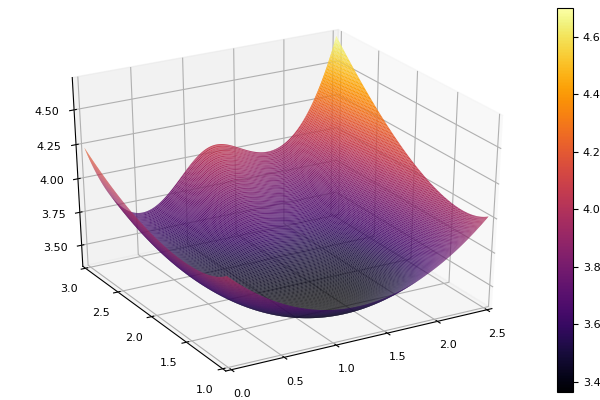
\includegraphics[scale=0.5]{surfacea.png}
    \end{center}
    \column{0.4\textwidth}
    \begin{itemize}
      \item[*] Max: 4.700
      \item[*] Min: 3.365
      \vspace{5mm}
      \item PSO result
      \item[] Nested PSO:  4.014
      \item[] Simple PSO: 4.700
    \end{itemize}
  \end{columns}
\end{frame}

\begin{frame}{Nested PSO, case (b)}
  \begin{flalign*}
    -log \hspace{1mm} det \left( \mathcal{I} \left( \xi^*,\theta^* \right) \right) = \min_{\xi \in \mathcal{X}} \max_{\theta \in \Theta} \left\{\hspace{1mm} -log \hspace{1mm} det \left( \mathcal{I} \left( \xi,\theta \right) \right) \hspace{1mm}\right\}
  \end{flalign*}
  Results, case (b) :\\
  \vspace{3mm}
  \begin{itemize}
    \item \makebox[2cm][l]{Outer loop} support($\xi_i^*$): -0.28, 0.66, 1.93, 2.88, 3,79, 5
    \item[] \makebox[2cm][l]{} weight($w_i^*$): 0.19, 0.25, 0.22, 0.18, 0.16, 0
    \vspace{3mm}
    \item \makebox[2cm][l]{Inner loop} parameter($\theta^*$): 0, 3.5
    \vspace{3mm}
    \item \makebox[2cm][l]{Optimum} $-log \hspace{1mm} det \left( \mathcal{I} \left( \xi^*,\theta^* \right) \right)=4.74$
  \end{itemize}
  \vspace{3mm}
  Design is also not symmetric.
\end{frame}

\begin{frame}{Nested PSO, case (b)}
  Plotting $-log \hspace{1mm} det \left( \mathcal{I} \left( \xi^*,\theta \right) \right)$ as a function of $\theta$\\
  \begin{columns}
    \column{0.6\textwidth}
    \begin{center}
      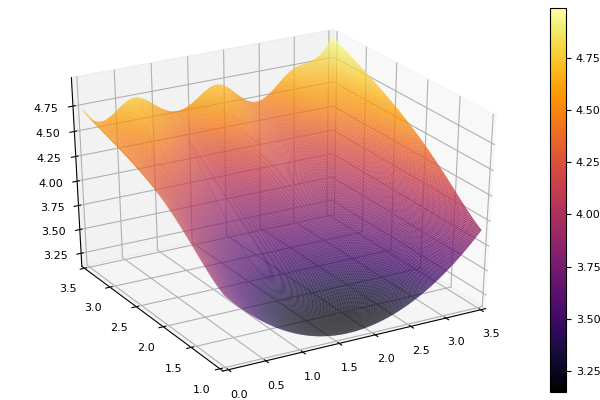
\includegraphics[scale=0.5]{surfaceb.png}
    \end{center}
    \column{0.4\textwidth}
    \begin{itemize}
      \item[*] Max: 4.989
      \item[*] Min: 3.149
      \vspace{5mm}
      \item PSO result
      \item[] Nested PSO: 4.740
      \item[] Simple PSO: 4.989
    \end{itemize}
  \end{columns}
\end{frame}

\begin{frame}{Symmetric Design Constraint, case (a)}
  Include symmetric design constraint in the PSO algorithm\\
  \vspace{3mm}
  Results, case (a) :\\
  \vspace{3mm}
  \begin{itemize}
    \item \makebox[2cm][l]{Outer loop} support($\xi_i^*$): -0.446282, 0.59195, 1.90805, 2.946282
    \item[] \makebox[2cm][l]{} weight($w_i^*$): 0.249949, 0.250051, 0.250051, 0.249949
    \vspace{3mm}
    \item \makebox[2cm][l]{Inner loop} parameter($\theta^*$): 2.5, 3
    \vspace{3mm}
    \item \makebox[2cm][l]{Optimum} $-log \hspace{1mm} det \left( \mathcal{I} \left( \xi^*,\theta^* \right) \right)=4.225$
  \end{itemize}
\end{frame}

\begin{frame}{Symmetric Design Constraint, case (a)}
  Plotting $-log \hspace{1mm} det \left( \mathcal{I} \left( \xi^*,\theta \right) \right)$ as a function of $\theta$\\
  \begin{columns}
    \column{0.6\textwidth}
    \begin{center}
      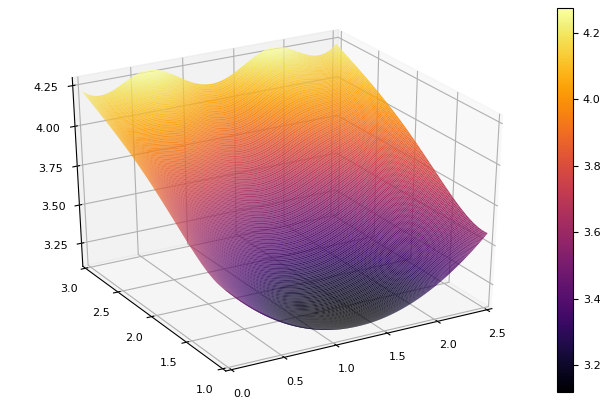
\includegraphics[scale=0.5]{surfacea_sym.png}
    \end{center}
    \column{0.4\textwidth}
    \begin{itemize}
      \item[*] Max: 4.275
      \item[*] Min: 3.120
      \vspace{5mm}
      \item PSO result
      \item[] Nested PSO: 4.225
      \item[] Simple PSO: 4.275*
      \item[] $\ast$: with 80\% chance
    \end{itemize}
  \end{columns}
\end{frame}

\begin{frame}{Symmetric Design Constraint, case (a)}
  Consider relative efficiency against the worst case scenario:
  \begin{align*}
    RE(\xi) =  \frac{\max_{\theta\in\Theta}\left\{\lvert Cov(\hat{\beta}(\xi^*,\theta))\rvert\right\}}{\max_{\theta\in\Theta}\left\{\lvert Cov(\hat{\beta}(\xi,\theta))\rvert\right\} }
  \end{align*}
  RE of nested PSO = 
  
\end{frame}

\begin{frame}{Symmetric Design Constraint, case (b)}
  \begin{flalign*}
    -log \hspace{1mm} det \left( \mathcal{I} \left( \xi^*,\theta^* \right) \right) = \min_{\xi \in \mathcal{X}} \max_{\theta \in \Theta} \left\{\hspace{1mm} -log \hspace{1mm} det \left( \mathcal{I} \left( \xi,\theta \right) \right) \hspace{1mm}\right\}
  \end{flalign*}
  Results, case (b) :\\
  \vspace{3mm}
  \begin{itemize}
    \item \makebox[2cm][l]{Outer loop} support($\xi_i^*$): -0.28, 0.66, 1.93, 2.88, 3,79, 5
    \item[] \makebox[2cm][l]{} weight($w_i^*$): 0.19, 0.25, 0.22, 0.18, 0.16, 0
    \vspace{3mm}
    \item \makebox[2cm][l]{Inner loop} parameter($\theta^*$): 0, 3.5
    \vspace{3mm}
    \item \makebox[2cm][l]{Optimum} $-log \hspace{1mm} det \left( \mathcal{I} \left( \xi^*,\theta^* \right) \right)=4.74$
  \end{itemize}
  \vspace{3mm}
  Design is also not symmetric.
\end{frame}

\begin{frame}{Symmetric Design Constraint, case (b)}
  Plotting $-log \hspace{1mm} det \left( \mathcal{I} \left( \xi^*,\theta \right) \right)$ as a function of $\theta$\\
  \begin{columns}
    \column{0.6\textwidth}
    \begin{center}
      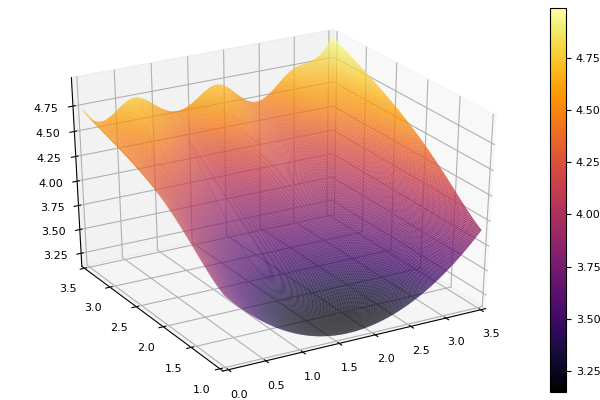
\includegraphics[scale=0.5]{surfaceb.png}
    \end{center}
    \column{0.4\textwidth}
    \begin{itemize}
      \item[*] Max: 4.989
      \item[*] Min: 3.149
      \vspace{5mm}
      \item PSO result
      \item[] Nested PSO: 4.740
      \item[] Simple PSO: 4.989
    \end{itemize}
  \end{columns}
\end{frame}

\begin{frame}{Learning Parameter}
    Fixed learning paramter $\gamma_1, \gamma_2=2$ might not fit every problem.\\
  \vspace{3mm}
  Compartment model example: $\mathcal{X}=[0,30]$\\
  Two-parameter logistic regression example: $\mathcal{X}=[-1,4]$ and $[-5,5]$.\\
  \vspace{3mm}
  The scale of $w$ in probability simplex does not vary.\\
  \vspace{3mm}
  Since $\gamma$ determines the diameter of particle movement in each iteration, learning parameter should be chosen according to the design space.\\
  \vspace{3mm}
  Inadequately large $\gamma$ will make the particles move only along the boundary.
\end{frame}

\begin{frame}{False Positive Error}
  Example 1 showed PSO algorithm may fail to find the global optimum.\\
  \vspace{3mm}
  Suppose, inner loop PSO algorithm fails and returns false $f_{outer}(u^x)$.\\
  \vspace{3mm}
  If $f_{outer}(u^x)$ is smaller than the current best position,\\
  $u_F$ and $f_{outer}(u_F)$ is saved in the solution path through the entire iteration.\\
  \vspace{3mm}
  The output we observe is a nonexistent minimax point.\\
  \vspace{3mm}
  Consider a simple setting where such failure occurs with probability $p$.\\
  Probability of a obtaining a solution free of $f_{outer}(u^x)$ after $n$ iteration is $\left(1-(1-p)^n\right)$.\\
  \vspace{3mm}
  Large number of iteration in nested PSO guarantees failure.\\
  \vspace{3mm}
  Nested PSO algorithm is not suitable for minimax optimization problem.
\end{frame}

\begin{frame}{Stability Inside the Inner Loop}
  Case (a): 1000 inner loop PSO simulation at $\xi^*$\\
  \begin{columns}
    \column{0.7\textwidth}
    \begin{center}
      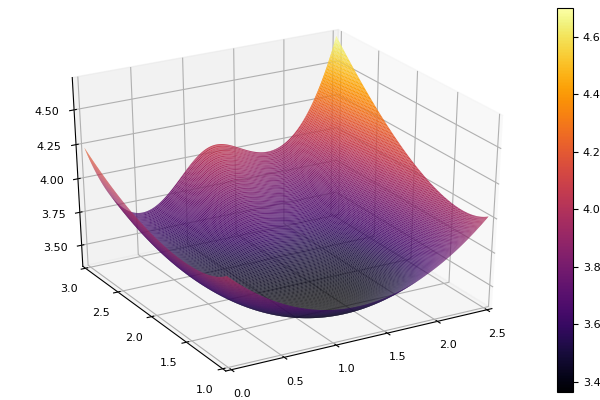
\includegraphics[scale=0.5]{surfacea.png}
    \end{center}
    \column{0.3\textwidth}
    \begin{itemize}
      \item[(1)] global max.
      \item[] $4.700$ $[2.5,3]$
      \item[(2)] local max:
      \item[] $4.233$ $[0,3]$
      \vspace{5mm}
      \item[] PSO Result
      \item[(1)] 95\% 
      \item[(2)] 5\%
    \end{itemize}
  \end{columns}
\end{frame}

\begin{frame}{Stability Inside the Inner Loop}
  Case (b): 1000 inner loop PSO simulation at $\xi^*$\\
  \begin{columns}
    \column{0.7\textwidth}
    \begin{center}
      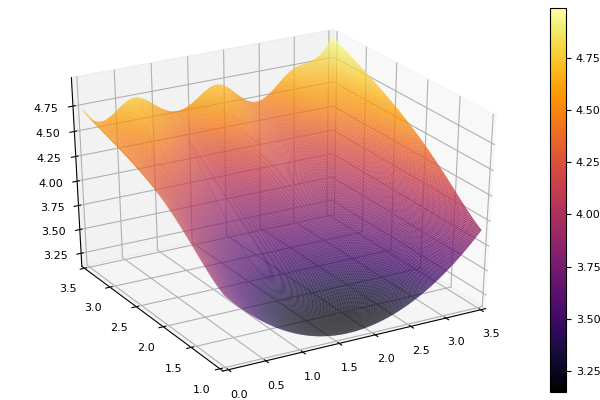
\includegraphics[scale=0.5]{surfaceb.png}
    \end{center}
    \column{0.3\textwidth}
    \begin{itemize}
      \item[(1)] global max.
      \item[] $4.989$ $[3.5,3.5]$
      \item[(2)] local max:
      \item[] $4.740$ $[0,3.5]$
      \vspace{5mm}
      \item[] PSO Result
      \item[(1)] 99.8\% 
      \item[(2)] 0.2\%
    \end{itemize}
  \end{columns}
\end{frame}

\begin{frame}{Modified Nested PSO}
  Since instability of simple PSO can raise a false alarm,\\
  nested PSO that double checks before solution update may perform better.
  \begin{flalign*}  
    \text{(1) }&\text{Initialize particles}\\
    \text{(2) }&\text{Repeat until stopping criteria are satisfied,}\\
    &\text{(2.1) Calculate particle velocity with Eq. (1)}\\
    &\text{(2.2) Update particle position with Eq. (2)}\\
    &\text{(2.3) Project particle back to design space}\\
    &\text{(2.4) Calculate } f_{outer}(x_i) \text{ via Algorithm (1) } \\
    &\text{(2.5)  \color{red}Check for failure} \text{ and update best positions } p_i, p_g \\
    \text{(3) }&\text{Output } p_g = \argmin_{u \in \mathcal{U}}\left\{ f_{outer}(u) \right\} \text{with \emph{gbest}}=f_{outer}  (p_g)
  \end{flalign*}
\end{frame}

\begin{frame}{Modified Nested PSO}
  Results, Example 2 case (a):\\
  \vspace{3mm}
  Double check before global update\\
  \vspace{1mm}
  \begin{itemize}
    \item \makebox[2cm][l]{Outer loop} support($\xi_i^*$): -1, 0.51, 1.70, 3.22
    \item[] \makebox[2cm][l]{} weight($w_i^*$): 0.21, 0.14, 0.54, 0.11
    \vspace{1mm}
    \item \makebox[2cm][l]{Inner loop} parameter($\theta^*$): 2.5, 1
  \end{itemize}
  \vspace{3mm}  
  Double check before personal and global update\\
  \vspace{1mm}
  \begin{itemize}
    \item \makebox[2cm][l]{Outer loop} support($\xi_i^*$): -0.22, 0.52, 1.89, 2.82
    \item[] \makebox[2cm][l]{} weight($w_i^*$): 0.31, 0.15, 0.32, 0.22
    \vspace{1 mm}
    \item \makebox[2cm][l]{Inner loop} parameter($\theta^*$): 1.77, 3
  \end{itemize}
  \vspace{3mm}
  As long as "double check" is stochastic, modified nested PSO also fails.
\end{frame}

\begin{frame}{Reference}
  \begin{itemize}
    \item Berger, M. P., \& Wong, W. K. (2009). An introduction to optimal designs for social and biomedical research (Vol. 83). John Wiley \& Sons.
    \item Chen, R. B., Chang, S. P., Wang, W., Tung, H. C., \& Wong, W. K. (2015). Minimax optimal designs via particle swarm optimization methods. Statistics and Computing, 25(5), 975-988.
    \item Berger, M. P., King, C. J., \& Wong, W. K. (2000). Minimax D-optimal designs for item response theory models. Psychometrika, 65(3), 377-390.
    \item King, J., \& Wong, W. K. (2000). Minimax D‐optimal designs for the logistic model. Biometrics, 56(4), 1263-1267.
    \item Qiu, J., Chen, R. B., Wang, W., \& Wong, W. K. (2014). Using animal instincts to design efficient biomedical studies via particle swarm optimization. Swarm and evolutionary computation, 18, 1-10.
  \end{itemize}
\end{frame}


%%%%%%%%%%%%%%%%%%%%%%%%%%%%%%%%%%%%%%%%%%%%%%%%%%%%%%%%%%


% Placing a * after \section means it will not show in the
% outline or table of contents.

%\section*{Summary}
%
%\begin{frame}{Summary}
%  \begin{itemize}
%  \item
%    The \alert{first main message} of your talk in one or two lines.
%  \item
%    The \alert{second main message} of your talk in one or two lines.
%  \item
%    Perhaps a \alert{third message}, but not more than that.
%  \end{itemize}
%  
%  \begin{itemize}
%  \item
%    Outlook
%    \begin{itemize}
%    \item
%      Something you haven't solved.
%    \item
%      Something else you haven't solved.
%    \end{itemize}
%  \end{itemize}
%\end{frame}



% All of the following is optional and typically not needed. 

%\appendix
%\section<presentation>*{\appendixname}
%\subsection<presentation>*{For Further Reading}

%\begin{frame}[allowframebreaks]
%  \frametitle<presentation>{For Further Reading}
    
%  \begin{thebibliography}{10}
    
%  \beamertemplatebookbibitems
  % Start with overview books.

%  \bibitem{Author1990}
%    A.~Author.
%    \newblock {\em Handbook of Everything}.
%    \newblock Some Press, 1990.
 
    
%  \beamertemplatearticlebibitems
  % Followed by interesting articles. Keep the list short. 

%  \bibitem{Someone2000}
%    S.~Someone.
%    \newblock On this and that.
%    \newblock {\em Journal of This and That}, 2(1):50--100,
%    2000.
%  \end{thebibliography}
%\end{frame}

\end{document}

